\section{Evaluation}
\frame{\frametitle{Agenda} \tableofcontents[currentsection]}
\begin{frame}
\frametitle{Experimental Setup}
\doublerulesep 0.1pt
\begin{table}[htb]
  \centering
 \linespread{1.7}{ {\tiny
%  \caption{Machine configurations}\label{tb:machines}
\vspace{-3em}
  \begin{tabular}{p{2.0cm}p{2.5cm}p{2.5cm}p{2.5cm}}
  \hline
\noalign{\smallskip}
    \textbf{Machine} & \textbf{PC A}&\textbf{PC B}&\textbf{PC C}\\
\noalign{\smallskip}
  \hline
    GPU&NVIDIA GTX280& NVIDIA 8800GTX & ATI Radeon HD 3870\\
    \# GPU core & 240 & 128 & 320 \\
    GPU Core Clock&602 MHz&575 MHz&775 MHz\\
    GPU Memory Clock&1107 MHz&900 MHz&2250 MHz \\
    GPU Memory Bandwidth& 141.7 GB/s& 86.4 GB/s&72.0 GB/s\\
    GPU Memory size& 1024 MB& 768 MB& 512 MB\\
    CPU&Intel Core2 Quad Q6600 & Intel Core2 Quad Q6600 & Intel Pentium 4 540 \\
    CPU Clock&2400 MHz&2400 MHz&3200 MHz\\
    \# CPU core& 4 & 4 & 2\\
    CPU Memory size& 2048 MB& 2048 MB& 1024 MB\\
    OS& 32-bit CentOS Linux& 32-bit CentOS Linux& 32-bit Windows XP\\
   \hline
 \hline
\noalign{\smallskip}
  \end{tabular}
  }}
\end{table}
\end{frame}

\begin{frame}
\frametitle{Applications}
\doublerulesep 0.1pt
\begin{table}[htb]
  \centering
 \linespread{1.7}{ {\tiny
%  \caption{The input data sizes of the micro-benchmark}\label{tab:app}
\vspace{-4em}
  \begin{tabular}{cp{2.5cm}p{2.5cm}p{2.5cm}}
  \hline
\noalign{\smallskip}
  \textbf{Applications} &  \textbf{Small} & \textbf{Medium} & \textbf{Large}\\
\noalign{\smallskip}
  \hline
  String Match (SM)  & size: 55MB & size: 105MB  & size: 160MB  \\
  Matrix Multiplication (MM)  & 256x256  &  512x512  &  1024x1024  \\
  Black-Scholes (BS) & \# option: 1,000,000  & \# option: 3,000,000  & \# option: 5,000,000  \\
  Similarity Score (SS) & \# feature: 128, \# documents: 512  & \# feature: 128, \# documents: 1024  & \# feature: 128, \# documents: 2048  \\
  PCA  & 1000x256  & 2000x256 &  4000x256  \\
  Monte Carlo (MC) & \# option: 500, \# samples per option: 500  &  \# option: 500, \# samples per option: 2500  &  \# option: 500, \# samples per option: 5000 \\
 \hline
\noalign{\smallskip}
  \end{tabular}
  }}
\end{table}
GPU Implementation: MarsCUDA, CUDA \\
CPU Implementation: MarsCPU, Phoenix, pthreads\\
GPU\-CPU Coprocessing: MarsCUDA + MarsCPU
\end{frame}

\subsection{Ease of use}
\begin{frame}
\frametitle{Code size saving}
In lines:
\doublerulesep 0.1pt
\begin{table}[htb]
  \centering
 \linespread{1.7}{ {\tiny
%  \caption{Comparison of application code size on MarsCPU, MarsCUDA, Phoenix, and  CUDA.}\label{tab:codesize}
\vspace{2em}
  \begin{tabular}{cccc}
  \hline
\noalign{\smallskip}
  \textbf{Applications} & \textbf{Phoenix} & \textbf{MarsCUDA/MarsCPU} & \textbf{CUDA} \\
\noalign{\smallskip}
  \hline
    String Match & 206 &  147 & 157 \\
  Matrix Multiplication & 178 & 72 & 68\\
  Black-Scholes & 199 & 147 & 721 \\
  Similarity Score & 125 & 82 & 615 \\
  Principal component analysis & 297 &  168 & 583 \\
  Monte Carlo & 251 &  203& 359 \\
  \hline
  \end{tabular}
  }}
\end{table}


\end{frame}

\subsection{High Performance}
\begin{frame}
\frametitle{MarsCPU vs Phoenix}
\begin{columns}
\column{0.65\textwidth}
\begin{block}{Speedup $= T_{Phoenix} / T_{MarsCPU}$}
\includegraphics[width=1.0\textwidth]{figure/MarsCPU_Phoenix.eps}
\end{block}
\column{0.35\textwidth}
\begin{block}{Overhead of Phoenix}
\begin{itemize}
\item<2-> Always need Reduce stage.
\item<3-> Lock overhead.
\item<4-> Re-allocate buffer on the fly.
\item<5-> Insertion sort on static arrays. Call {\em memmove()} frequently.
\end{itemize}
\end{block}
\end{columns}
\end{frame}

\begin{frame}
\frametitle{MarsCUDA vs MarsCPU on Kernel}
\begin{columns}
\column{0.65\textwidth}
\begin{block}{Speedup $= T_{MarsCPU*} / T_{MarsCUDA*}$}
\includegraphics[width=1.0\textwidth]{figure/kernel.eps}
\end{block}
\column{0.35\textwidth}
\begin{itemize}
\item \sout{Preprocess} + \textbf{Map} + \sout{Group} + \textbf{Reduce}
\end{itemize}
\end{columns}
\end{frame}

\begin{frame}
\frametitle{MarsCUDA vs MarsCPU}
\begin{columns}
\column{0.65\textwidth}
\begin{block}{Speedup $= T_{MarsCPU} / T_{MarsCUDA}$}
\includegraphics[width=1.0\textwidth]{figure/MarsGPU_MarsCPU.eps}
\end{block}
\column{0.35\textwidth}
\begin{itemize}
\item Preprocess + Map + Group + Reduce
\end{itemize}
\end{columns}
\end{frame}

\begin{frame}
\frametitle{Time Breakdown}
\begin{columns}
\column{0.5\textwidth}
\begin{block}{MarsCUDA}
\includegraphics[width=1.0\linewidth]{figure/MarsGPU_Timebreakdown.eps}
\end{block}
\column{0.5\textwidth}
\begin{block}{MarsCPU}
\includegraphics[width=1.0\linewidth]{figure/MarsCPU_Timebreakdown.eps}
\end{block}
\end{columns}
\end{frame}

\begin{frame}
\frametitle{Amdahl's Law}
\begin{columns}
\column{0.50\textwidth}
\begin{block}{Amdahl's Law}
Speedup $= \frac{1}{(1 - P) + P/S}$
\begin{itemize}
\item $P$: The proportion that is parallelized
\item $(1 - P)$: The proportion that is not parallelized
\item $S$: Speedup by parallelism
\end{itemize}
\end{block}
\column{0.50\textwidth}
\begin{block}{For MarsCUDA}<2->
\begin{itemize}
\item P: Map + Reduce
\item (1 - P): Preprocess
\item Example: String Match
\begin{itemize}
\item Parallelized: Map stage
\item P $= 25\%$
\item S $= 20$
\item Speedup $= \frac{1}{(1 - 25\%)+25\%/20} = 1.3$
\end{itemize}
\end{itemize}
\end{block}
\end{columns}
\end{frame}

\begin{frame}
\frametitle{Preprocess is a bottleneck?}
Real world applications in Chained MapReduce:

\underline{Preprocess}$\rightarrow$Map1$\rightarrow$Group1$\rightarrow$Reduce1$\rightarrow$\textcolor{red}{Map2}$\rightarrow$\textcolor{blue}{Map3}$\rightarrow$\\
\textcolor{green}{Map4}$\rightarrow$\textcolor{green}{Group4}
\begin{itemize}
\item Prepare key/value pairs
\item Transfer input key/value pairs from main memory to device memory
\end{itemize}
\end{frame}


\begin{frame}
\frametitle{GPU/CPU Co-processing}
\begin{columns}
\column{0.65\textwidth}
\begin{block}{Speedup $= T_{Standalone}/T_{Coprocessing} $}
\includegraphics[width=1.0\textwidth]{figure/coprocess.eps}
\end{block}
\column{0.35\textwidth}
Co-processing over MarsCUDA:
\begin{itemize}
\item Speedup $= \frac{S+1}{S}$
\item $S$: Speedup of MarsCUDA over MarsCPU
\end{itemize}
\end{columns}
\end{frame}

\begin{frame}
\frametitle{MarsHadoop}
\begin{columns}
\column{0.5\textwidth}
\begin{block}{Speedup $= T_{Hadoop}/T_{MarsHadoop}$}
\includegraphics[width=1.00\linewidth]{figure/speeduphadoop.eps}
\end{block}
\column{0.5\textwidth}
\begin{block}{Time Breakdown}
\includegraphics[width=1.0\linewidth]{figure/breakdownhadoop.eps}
\end{block}
\end{columns}
Two slave nodes: PC A and PC B\\
One master node: PC A
\end{frame}
